\documentclass[10pt]{beamer}

\usepackage{polyglossia}
\usepackage{csquotes}
\usepackage{datetime}
\usepackage{fontspec}
\usepackage{microtype}
\usepackage{color}
\usepackage{url}
\usepackage{hyperref}
\usepackage{amsfonts}
\usepackage{amsmath}
\usepackage{amsthm}
\usepackage{subcaption}
\usepackage[backend=biber,style=iso-authoryear,sortlocale=en_US,autolang=other,bibencoding=UTF8]{biblatex}
\usepackage{booktabs}
\usepackage{graphics}

\addbibresource{zotero.bib}

\setdefaultlanguage{english}
\setmainfont{TeX Gyre Termes}
\usetheme{Boadilla}
\usecolortheme{crane}
\setbeamertemplate{title page}[default][rounded=true,shadow=false]
\setbeamertemplate{section in toc}[ball unnumbered]
\setbeamertemplate{bibliography item}{}

\hypersetup{
	pdfencoding=auto,
	unicode=true,
	citecolor=green,
	filecolor=blue,
	linkcolor=red,
	urlcolor=blue
}

\makeatletter
\newcommand*{\currentSection}{\@currentlabelname}
\makeatother

\newcommand{\mathmat}{\ensuremath{\mathbf}}

\title[Multi-instance clustering]
{
	Loss Functions for Clustering in Multi-instance Learning
}

\newdate{presentation}{21}{09}{2020}
\date[ITAT 2020]{ITAT 2020, \displaydate{presentation}}

\author[Marek Dědič]
{
	\underline{Marek~Dědič}\inst{1}\inst{2},
	Tomáš~Pevný\inst{3},
	Lukáš~Bajer\inst{2},
	Martin~Holeňa\inst{4}
}

\institute[ČVUT \& Cisco]
{
	\inst{1} Faculty of Nuclear Sciences and Physical Engineering, Czech Technical University in Prague \and
	\inst{2} Cisco Systems, Inc. \and
	\inst{3} Faculty of Electrical Engineering, Czech Technical University in Prague \and
	\inst{4} Institute of Computer Science, Czech Academy of Sciences
}

\AtBeginSection[]{
	\begin{frame}{\currentSection}
		\tableofcontents[currentsection]
	\end{frame}
}

\begin{document}

\begin{frame}
	\titlepage
\end{frame}

% Body

\section{Motivation \& Solved problem}

\begin{frame}{Motivation}
	\begin{itemize}
		\item Clustering is one of the basic problems solved with unsupervised machine learning.
		\item Trying to find a good metric for complex data is a key design element of their clustering.
		\item Multi-instance learning is a way of creating complex hierarchical models tailored to a specific problem at hand.
		\item 3 approaches for multi-instance clustering explored - CPC (unsupervised), Triplet loss, and Magnet loss (supervised)
	\end{itemize}
\end{frame}

\begin{frame}{Problem being solved}
	\begin{itemize}
		\item Computer network security is an attractive application for ML and presents complex data.
		\item The goal of our work was to enable clustering of second-level domains based on which clients connect to them.
		\item Clustering is very useful in this domain as it multiplies the work of network analysts.
	\end{itemize}
\end{frame}

\begin{frame}{Presentation outline}
	\tableofcontents
\end{frame}

\section{MIL}

\begin{frame}[c]\frametitle{Ordinary classification}
	\centering
	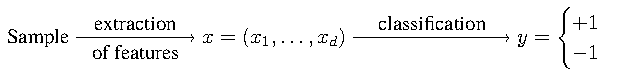
\includegraphics{images/end_to_end_learning/end_to_end_learning.pdf}
\end{frame}

\begin{frame}[c]\frametitle{Multi-instance classification}
	\centering
	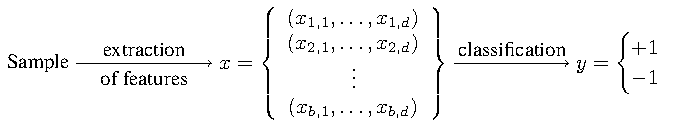
\includegraphics{images/multi_instance_learning/multi_instance_learning.pdf}
\end{frame}

\begin{frame}[c]\frametitle{Embedded space paradigm}
	\centering
	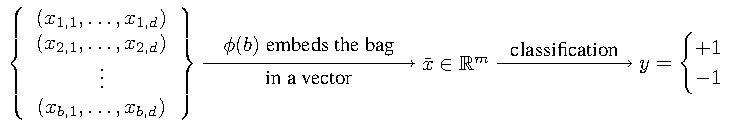
\includegraphics[width=0.9\pagewidth]{images/embedded_space_paradigm/embedded_space_paradigm.pdf}
\end{frame}

\begin{frame}{The embedding function \( \phi \)}
	\centering
	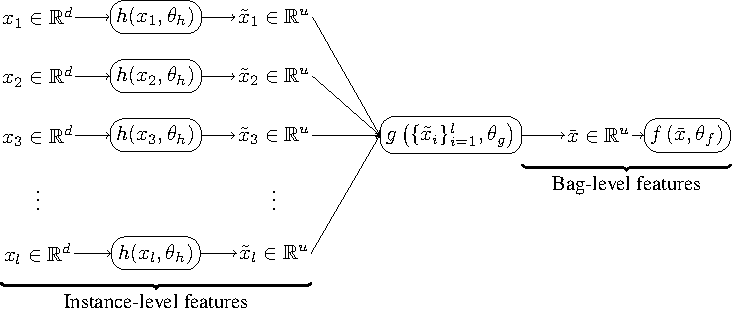
\includegraphics[width=0.9\pagewidth]{images/embedding_function/embedding_function.pdf}
\end{frame}

\section{Contrastive predictive coding}

\begin{frame}{Contrastive predictive coding}
	The approach based on Contrastive Predictive Coding is represented with the loss function \( L_\mathrm{CPC} \):
	\[ \mathmat{D}_{ij} = \left\lVert \phi \left( B_i^{(1)} \right) - \phi \left( B_j^{(2)} \right) \right\rVert_2^2 \]
	\[ L_\mathrm{CPC} = \frac{1}{n} \sum_{i = 1}^n \left( \log \left( \mathmat{D}_{ii} \right) - \log \sum_{\substack{j = 1 \\ j \neq i}}^n \mathmat{D}_{ij} \right) \]
\end{frame}

\section{Triplet loss}

\begin{frame}{Triplet loss}
	Triplet loss is a supervised alternative:
	\[ \mathmat{y}_{ij} =
		\begin{cases}
			1 &\text{for} \quad y_i = y_j \\
			0 &\text{otherwise}
		\end{cases}
	\]
	\[ \mathmat{\eta}_{ij} = \begin{cases}
		1 &\text{if the bag } B_j \text{ is a target neighbour of the bag } B_i \\
		0 &\text{otherwise}
	\end{cases} \]
	\[ L_\mathrm{triplet} = \sum_{ij} \eta_{ij} \mathmat{D}_{ij} + c \sum_{ijl} \eta_{ij} \left( 1 - \mathmat{y}_{il} \right) \max \left( 0, 1 + \mathmat{D}_{ij} - \mathmat{D}_{il} \right) \]
\end{frame}

\section{Magnet loss}

\begin{frame}{Magnet loss}
	\begin{figure}[h]
		\centering
		\begin{subfigure}[b]{0.18\textwidth}
			\centering
			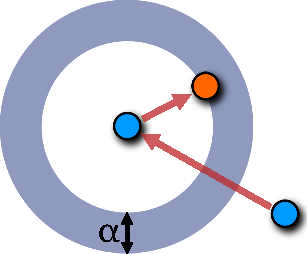
\includegraphics[width=\textwidth]{images/triplet-magnet-difference/triplet_before.pdf}
			\caption{Triplet loss: before}
		\end{subfigure}
		\hfill
		\begin{subfigure}[b]{0.18\textwidth}
			\centering
			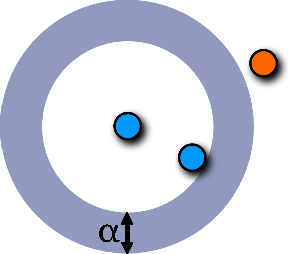
\includegraphics[width=\textwidth]{images/triplet-magnet-difference/triplet_after.pdf}
			\caption{Triplet loss: after}
		\end{subfigure}
		\hfill
		\begin{subfigure}[b]{0.18\textwidth}
			\centering
			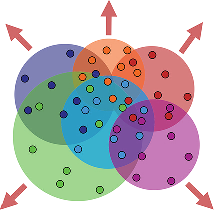
\includegraphics[width=\textwidth]{images/triplet-magnet-difference/magnet_before.pdf}
			\caption{Magnet loss: before}
		\end{subfigure}
		\hfill
		\begin{subfigure}[b]{0.18\textwidth}
			\centering
			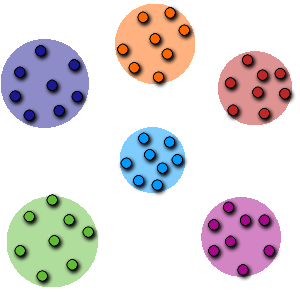
\includegraphics[width=\textwidth]{images/triplet-magnet-difference/magnet_after.pdf}
			\caption{Magnet loss: after}
		\end{subfigure}
		\caption{Visualization of the difference between triplet and magnet loss. Image from \cite{rippel_metric_2016}.}
	\end{figure}
\end{frame}

\section{Results on public datasets}

\begin{frame}{Publicly available datasets}
	\begin{figure}
		\centering
		\begin{subfigure}[t]{0.38\textwidth}
			\centering
			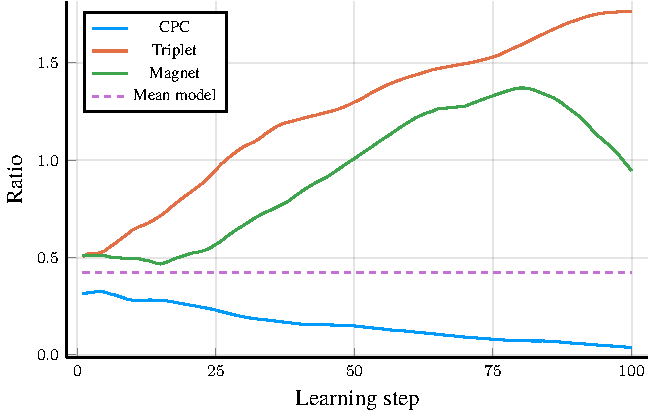
\includegraphics[width=\textwidth]{images/Musk2_ratio/Musk2_ratio.pdf}
			\caption{Musk2}
		\end{subfigure}
		\begin{subfigure}[t]{0.38\textwidth}
			\centering
			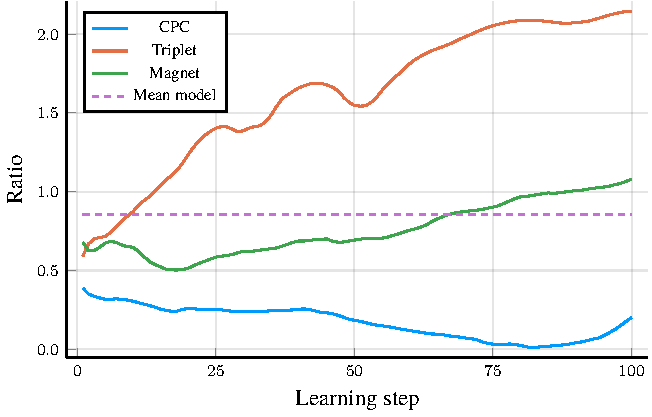
\includegraphics[width=\textwidth]{images/UCSBBreastCancer_ratio/UCSBBreastCancer_ratio.pdf}
			\caption{UCSBBreastCancer}
		\end{subfigure}
		\begin{subfigure}[t]{0.38\textwidth}
			\centering
			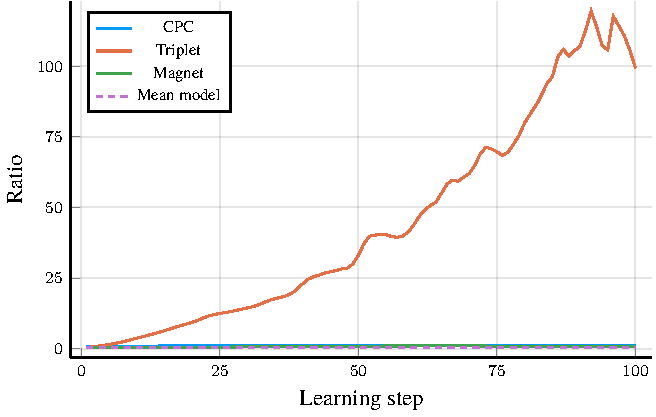
\includegraphics[width=\textwidth]{images/Web3_ratio/Web3_ratio.pdf}
			\caption{Web3}
		\end{subfigure}
		\caption{The Silhouette coefficient on three selected datasets.}
	\end{figure}
\end{frame}

\begin{frame}{Publicly available datasets}
	\begin{table}[h!]
		\centering
		\resizebox{!}{0.39\textheight}{%
			\begin{tabular}{lrrr}
				\toprule
				Dataset          & CPC            & Triplet loss   & Magnet loss \\
				\midrule
				BrownCreeper     & \textbf{0.900} & 0.882          & \textbf{0.900} \\
				Elephant         & 0.575          & \textbf{0.900} & 0.825 \\
				Fox              & 0.400          & 0.675          & \textbf{0.725} \\
				Musk1            & 0.667          & \textbf{0.889} & \textbf{0.889} \\
				Musk2            & 0.750          & \textbf{0.950} & \textbf{0.950} \\
				Mutagenesis1     & 0.658          & 0.816          & \textbf{0.912} \\
				Mutagenesis2     & 0.708          & \textbf{1.000} & \textbf{1.000} \\
				Newsgroups1      & 0.533          & 0.950          & \textbf{1.000} \\
				Newsgroups2      & 0.600          & 0.900          & \textbf{0.950} \\
				Newsgroups3      & 0.683          & 0.700          & \textbf{0.850} \\
				Protein          & 0.820          & \textbf{0.923} & 0.897 \\
				Tiger            & 0.642          & \textbf{0.825} & \textbf{0.825} \\
				UCSBBreastCancer & 0.333          & 0.667          & \textbf{1.000} \\
				Web1             & 0.667          & 0.733          & \textbf{0.800} \\
				Web2             & 0.689          & \textbf{0.800} & 0.733 \\
				Web3             & 0.733          & 0.800          & \textbf{1.000} \\
				Web4             & 0.622          & 0.800          & \textbf{0.930} \\
				WinterWren       & 0.936          & \textbf{0.955} & 0.936 \\
				\bottomrule
			\end{tabular}%
		}
		\caption{The accuracy of a kNN classifier in the representation space}
	\end{table}
\end{frame}

\section{Results on a corporate dataset}

\begin{frame}{Model for second-level domains}
	\begin{figure}
		\centering
		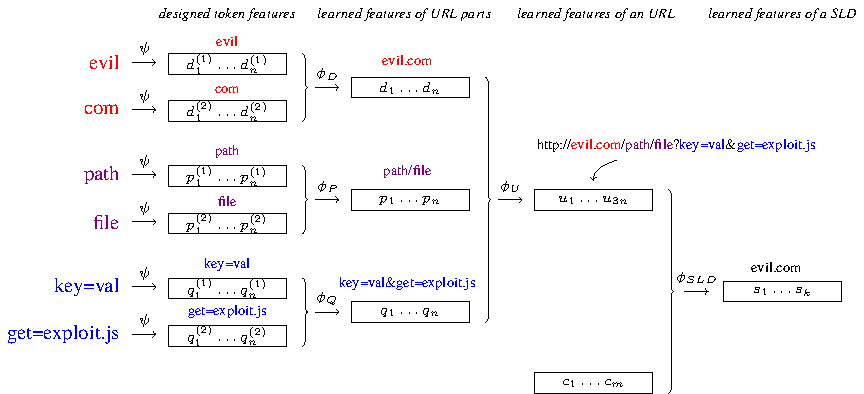
\includegraphics[width=\textwidth]{images/URL-model/URL-model.pdf}
	\end{figure}
\end{frame}

\begin{frame}{Corporate dataset results}
	\begin{table}
		\centering
		\begin{tabular}{lrrr}
			\toprule
			Variant    & CPC   & Triplet loss & Magnet loss \\
			\midrule
			2 classes  & 0.920 & 0.910        & \textbf{0.930} \\
			20 classes & 0.893 & 0.868        & \textbf{0.904} \\
			\bottomrule
		\end{tabular}
		\caption{The accuracy of a kNN classifier in the representation space}
	\end{table}
\end{frame}

\section{Conclusion}

\begin{frame}{Conclusion I.}
	\begin{itemize}
		\item We introduced and evaluated 3 approaches for MIL clustering.
		\item The approaches were compared on publicly available datasets and on a corporate dataset from the domain of computer network security.
		\item CPC performed poorly, moreover, it shows no clear improvement over the learning period.
	\end{itemize}
\end{frame}

\begin{frame}{Statistical significance}
	\begin{itemize}
		\item The null hypothesis that all three methods are the same as measured by the accuracy can be rejected at a 5 \% level of significance by the Friedman two-way analysis of variance by ranks.
		\item Triplet and magnet losses are better than CPC at a 5 \% level of significance by the post-hoc Nemenyi pairwise test.
		\item The null hypothesis that magnet loss and triplet loss are the same cannot be rejected at the 5 \% significance level by this test.
	\end{itemize}
\end{frame}

\begin{frame}{Conclusion II.}
	\begin{itemize}
		\item The comparison might not be fair, however, as the CPC method is unsupervised, whereas the other two can utilize labels on the training data, giving them a strong advantage.
		\item The initial expectation of CPC being outperformed proved to be true.
		\item These results are valuable in providing a comparison and a baseline for future work.
	\end{itemize}
\end{frame}

\begin{frame}
	\titlepage
\end{frame}

\end{document}
